\section{Results and Discussion}

\subsection{System Implementation and Live Lexicon}
The implemented \textit{Pinoy Speak} system is currently deployed as a full-stack web application with a FastAPI backend and a Next.js frontend. The system collects public text from Reddit, YouTube comments, and user chat interactions. As of the current implementation, the corpus contains 175,481 archived records: 163,372 Reddit records, 12,075 YouTube comments, and 34 chat interaction records.

The live lexicon contains approximately 104 verified slang entries. This includes 102 seed entries and dynamically discovered entries. Among the seed entries, 29 are marked as ambiguous because they require surrounding context before being classified as slang. These include words such as \textit{bet}, \textit{solid}, \textit{ghost}, \textit{slay}, \textit{sus}, \textit{chika}, and \textit{tropa}. The formal lexicon validation, however, covered 79 selected entries with three ratings per entry. This distinction is important because the live system contains both seed and dynamically discovered entries, while the validation set represents the subset formally reviewed by human validators.

The resulting system demonstrates the feasibility of maintaining a dynamic lexicon that combines seeded knowledge, corpus-based discovery, and LLM-assisted enrichment. The deployed application also integrates the core modules needed for slang exploration and learning, including the live dashboard, dictionary, tutor, translator, top slang leaderboard, concordance search, and about page. The frontend is hosted on Vercel, while the backend is hosted on Fly.io, allowing users to access the system through a browser without installing local software.

\subsection{Observed Reduction of False Positives}
Early system outputs showed that standard Tagalog inflected words could be incorrectly flagged as novel slang because they were unfamiliar to subword or dictionary checks. To address this, the system added a morphological prefix filter for common Filipino affix patterns such as \textit{naka-}, \textit{napaka-}, \textit{nag-}, and \textit{pinaka-}. This filtering step reduced observed false positives in candidate lists by excluding common standard Tagalog conjugations before novelty and burstiness checks.

A second source of false positives came from ambiguous English or Filipino words that can function as slang only in certain contexts. The context-window gate addresses this by checking nearby Filipino particles and intensifiers before confirming ambiguous entries. This allows the system to reject English-context uses such as ``I bet'' while still accepting Filipino-context uses of terms such as \textit{bet}, \textit{solid}, and \textit{grabe}. These controls improve the interpretability of the resulting lexicon, although a full before-and-after quantitative false-positive analysis remains part of future work.

\subsection{Detection of Semantic Shifts}
The system can identify known words that may be undergoing contextual or semantic shift. Instead of treating all dictionary words as non-candidates, the pipeline monitors known words for unusual increases in frequency. If a known term exceeds the semantic-shift threshold, it is flagged for review and enrichment.

Fig. \ref{fig:semantic-shift} presents a conceptual illustration of this process using the Filipino word \textit{buwaya}. In its literal meaning, \textit{buwaya} refers to a crocodile. In informal political discourse, however, it may be used figuratively to refer to corruption or greed. The figure is not presented as a direct output of a measured embedding experiment; rather, it illustrates how vector-space movement can represent a shift from literal to figurative contexts.

\begin{figure}[!t]
\centering
\resizebox{0.58\columnwidth}{!}{%
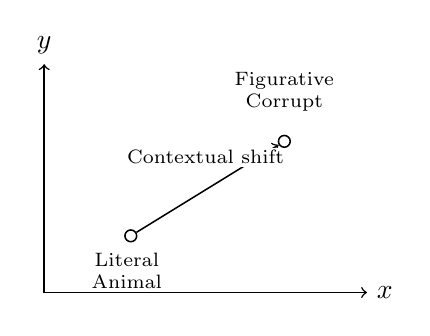
\begin{tikzpicture}[
    axis/.style={->, line width=0.55pt},
    shiftarrow/.style={->, line width=0.55pt},
    point/.style={circle, draw=black, fill=white, line width=0.55pt, inner sep=1.5pt},
    label/.style={font=\scriptsize, align=center}
]
    % Axes
    \draw[axis] (0,0) -- (4.1,0) node[right] {$x$};
    \draw[axis] (0,0) -- (0,2.9) node[above] {$y$};

    % Points
    \node[point] (literal) at (1.10,0.72) {};
    \node[point] (figurative) at (3.05,1.92) {};

    % Arrow
    \draw[shiftarrow] (literal) -- (figurative);

    % Labels
    \node[label] at (1.05,0.28) {Literal\\Animal};
    \node[label] at (3.05,2.55) {Figurative\\Corrupt};
    \node[label, fill=white, inner sep=1pt] at (2.05,1.72) {Contextual shift};
\end{tikzpicture}%
}
\caption{Conceptual illustration of semantic shift from literal to figurative usage.}
\label{fig:semantic-shift}
\end{figure}

\subsection{Interactive Chatbot and RAG-Grounded Explanations}
The ``Kuya Slang'' tutor, accessed through the \texttt{/tutor} route, provides conversational explanations of slang terms. Unlike the enrichment pipeline, which is used for generating dictionary entries, the tutor uses a separate chatbot LLM stack and retrieves relevant entries from the live lexicon before answering. This retrieval step helps ground responses in verified dictionary content and reduces the risk of unsupported explanations.

The tutor is particularly useful for learners who need more than a one-word definition. It can explain usage, give examples, and clarify the difference between literal and slang meanings. This supports the educational goal of the system by turning the lexicon into an interactive learning resource rather than a static list.

\subsection{Lexicon Validation Results}
A separate lexicon validation was conducted to determine whether the system-generated dictionary entries were acceptable to Filipino or Taglish speakers. The validation covered 79 slang entries across three form parts, with each entry receiving three item-level ratings. This produced 237 total item-level judgments. Although four unique validators participated across the form parts, each lexical item was still evaluated by three validators.

Overall results were positive. Validators marked 227 of 237 item-level judgments (95.78\%) as actually used in Filipino or Taglish slang. Definition correctness obtained a mean score of 4.83 out of 5, while example sentence naturalness obtained a mean score of 4.75 out of 5. Formation type acceptability was marked ``Yes'' in 222 of 237 judgments (93.67\%). Final entry judgments were also favorable: 208 of 237 judgments (87.76\%) were marked as correct or acceptable, 23 (9.70\%) needed minor revision, and 6 (2.53\%) were marked as incorrect or possible false positives.

\begin{table}[!t]
\centering
\caption{Summary of Lexicon Validation Results}
\label{tab:lexicon-validation}
\scriptsize
\setlength{\tabcolsep}{4pt}
\begin{tabular}{lc}
\toprule
\textbf{Validation Metric} & \textbf{Result} \\
\midrule
Validated slang entries & 79 \\
Total item-level ratings & 237 \\
Actually used as slang & 95.78\% \\
Definition correctness & 4.83 / 5 \\
Example naturalness & 4.75 / 5 \\
Formation type acceptable & 93.67\% \\
Final judgment: correct/acceptable & 87.76\% \\
Final judgment: needs minor revision & 9.70\% \\
Final judgment: incorrect/false positive & 2.53\% \\
\bottomrule
\end{tabular}
\end{table}

At the word level, 55 of 79 entries received unanimous correct or acceptable judgments from all three validators. Twenty entries received two correct or acceptable judgments and one revision or rejection judgment. Four entries received one or fewer correct judgments: \textit{basic}, \textit{dead}, \textit{dogshow}, and \textit{yarn}. These entries require priority revision because validator comments indicated possible definition mismatch or insufficient contextual explanation. For instance, validators noted that \textit{dogshow} is more accurately understood as playful teasing, mocking, or making fun of someone, while \textit{yarn} should be explained as a stylized form of \textit{iyan} or \textit{yan} rather than treated as a completely independent lexical origin.

Validator comments also showed that some terms are acceptable as entries but require metadata corrections. Examples include \textit{bonak}, whose formation was described as a contraction related to \textit{bobong anak}; \textit{omsim} and \textit{lodi}, which should be consistently labeled as reversed forms; and borrowed English items such as \textit{legit}, \textit{savage}, \textit{shook}, and \textit{shookt}, whose formation labels should more clearly identify borrowing or semantic shift. These comments are important because they show that system accuracy is not limited to meaning alone; origin, formation type, and example naturalness also affect lexicon quality.

\subsection{User Evaluation Results}
A usability evaluation survey was conducted as a beta evaluation to assess the usability, clarity, perceived usefulness, and bug behavior of the deployed \textit{Pinoy Speak} web application. The survey received 39 submissions. After excluding two non-consenting responses and one blank-consent response, 36 valid responses were retained. Respondents came from several age groups, with 18--24 as the largest group (17 respondents), followed by 25--34 (9 respondents), 45 and above (4 respondents), under 18 (4 respondents), and 35--44 (2 respondents). The respondent group included 18 students, 15 employed users, and three respondents from other categories. Windows was the most frequently used operating system, while Chrome was the most frequently used browser.

The beta evaluation used task-based testing to check whether users could interact with the major modules of the system. One example task involved the Analyzer or Translator module, where users could enter a Taglish sentence such as ``Bet ko itong outfit mo, sobrang solid.'' This example tested whether the system could interpret ambiguous slang expressions using context. In this case, \textit{bet} should be interpreted as approval or preference in a Filipino or Taglish sentence, while \textit{solid} may function as an informal positive description. The expected output was that the Analyzer or Translator would identify these terms as informal Taglish expressions based on surrounding Filipino context words such as \textit{ko}, \textit{itong}, and \textit{mo}. This example shows that the beta evaluation did not only measure interface usability but also tested whether the system could support contextual slang understanding.

Across the evaluated modules, the application received high usability scores. As shown in Table \ref{tab:module-usability}, the Dictionary module obtained the highest average overall usability score at 9.36 out of 10, followed by the Tutor module at 9.33, Navigation Flow at 9.14, Analyzer or Translator at 9.00, Top Slang or Usage Frequency at 8.85, and Dashboard or Word Popularity at 8.58. These results suggest that users found the core lexicon and learning-oriented features especially usable. The Analyzer or Translator score of 9.00 out of 10 also supports the usefulness of including concrete beta testing tasks involving contextual slang interpretation.

\begin{table}[!t]
\centering
\caption{Module-Level Usability and Quality Ratings}
\label{tab:module-usability}
\scriptsize
\setlength{\tabcolsep}{2.5pt}
\begin{tabular}{p{0.35\columnwidth}cccc}
\toprule
\textbf{Module / Task} & \textbf{Use.} & \textbf{Aes.} & \textbf{Spd.} & \textbf{Acc.} \\
\midrule
Dashboard / Word Popularity & 8.58 & 4.33 & 4.47 & 4.25 \\
Navigation / Menu Flow & 9.14 & 4.53 & 4.44 & 4.42 \\
Top Slang / Usage Frequency & 8.85 & 4.50 & 4.56 & 4.33 \\
Dictionary / Word Cards & 9.36 & 4.47 & 4.50 & 4.33 \\
Analyzer / Translator & 9.00 & 4.64 & 4.53 & 4.42 \\
Tutor / Chatbot & 9.33 & 4.58 & 4.61 & 4.44 \\
\bottomrule
\end{tabular}
\vspace{2pt}
\begin{flushleft}
\scriptsize
\textit{Note.} Use. = usability; Aes. = aesthetics; Spd. = speed; Acc. = data accuracy.
\end{flushleft}
\end{table}

Bug reports were generally low, but they identify practical areas for refinement. The Dashboard or Word Popularity module received the highest number of bug reports at 6 of 36 responses (16.67\%), followed by the Top Slang or Usage Frequency module with 4 reports (11.11\%). The remaining evaluated modules each received only one bug report. Reported issues included unclear zooming in charts, delayed or missing chart rendering, search behavior in the dictionary, minor animation shifts in the analyzer, and occasional tutor-answer mismatches.

\begin{table}[!t]
\centering
\caption{Reported Bug Occurrence by Module}
\label{tab:bug-results}
\scriptsize
\setlength{\tabcolsep}{4pt}
\begin{tabular}{p{0.48\columnwidth}cc}
\toprule
\textbf{Module / Task} & \textbf{Reports} & \textbf{Percent} \\
\midrule
Dashboard / Word Popularity & 6 & 16.67\% \\
Navigation / Menu Flow & 1 & 2.78\% \\
Top Slang / Usage Frequency & 4 & 11.11\% \\
Dictionary / Word Cards & 1 & 2.78\% \\
Analyzer / Translator & 1 & 2.78\% \\
Tutor / Chatbot & 1 & 2.78\% \\
\bottomrule
\end{tabular}
\end{table}

At the general application level, respondents gave strong ratings for readability, navigation, usefulness, and recommendation. The interface was rated visually clear and readable at 4.72 out of 5, while ease of navigation was rated 4.67 out of 5. The Dictionary was rated 4.61 out of 5 for usefulness, and the recommendation item also received 4.61 out of 5. The application helped users understand the context of slang, not just its meaning, with a mean rating of 4.50 out of 5. In addition, 31 of 36 respondents (86.11\%) reported that they learned at least one new slang word or expression from the application.

\begin{table}[!t]
\centering
\caption{General Application-Level Evaluation Results}
\label{tab:general-evaluation}
\scriptsize
\setlength{\tabcolsep}{3pt}
\begin{tabular}{p{0.72\columnwidth}c}
\toprule
\textbf{Evaluation Item} & \textbf{Mean} \\
\midrule
Interface was visually clear and readable & 4.72 / 5 \\
App was easy to navigate & 4.67 / 5 \\
Dictionary was useful & 4.61 / 5 \\
Would recommend Pinoy Speak & 4.61 / 5 \\
Helped understand slang context & 4.50 / 5 \\
Tutor helped users understand slang & 4.42 / 5 \\
Definitions/examples felt accurate and natural & 4.25 / 5 \\
Improved confidence in understanding slang & 4.25 / 5 \\
Compared favorably with other slang-learning sources & 3.94 / 5 \\
\bottomrule
\end{tabular}
\end{table}

The most frequently selected useful features were the Dictionary and the overall feature set, with 12 selections each. Other useful features included Concordance, Chat Tutor, Translator, and Top Slang. Qualitative feedback emphasized the need to expand the slang vocabulary, improve selected definitions and translations, add pronunciation support, include regional Philippine languages or slang varieties, freeze or improve dictionary navigation controls, clarify chart interactions, and separate quiz or flashcard activities from the tutor interface.

Overall, the beta evaluation results indicate that the deployed application is usable for its intended users and that the main learning-oriented modules are understandable. However, the feedback also shows that the application still requires iterative improvement, especially in expanding the slang database, refining selected definitions and translations, improving chart interactions, and reducing occasional tutor-answer mismatches.

\subsection{Discussion}
The results show that \textit{Pinoy Speak} addresses the main problem identified in this study: informal Filipino and Taglish evolve faster than static dictionaries and conventional NLP tools can accommodate. The implemented system responds to this problem by combining corpus-based trend detection, contextual classification, LLM-assisted enrichment, and user-facing educational modules.

The lexicon validation results support the usefulness of the dictionary, but they also show that a dynamic lexicon requires human review. High definition and example scores indicate that most entries are understandable and natural. However, the minor revision and false-positive judgments show that some entries need stronger distinction between slang, ordinary Filipino vocabulary, borrowed English usage, and context-dependent semantic shift. This is especially important for entries such as \textit{bawi}, \textit{malas}, \textit{swerte}, \textit{tampo}, and \textit{wagi}, where validators questioned whether the word is slang or standard vocabulary.

The usability and beta evaluation results show that users value the Dictionary, Tutor, and Analyzer modules. These modules directly support the educational aim of the project because they help users look up meanings, see examples, and ask follow-up questions. The beta testing example using a Taglish sentence such as ``Bet ko itong outfit mo, sobrang solid'' also demonstrates why context-aware analysis is necessary. The system must not only detect individual slang terms but also interpret them based on the surrounding words. However, the lower ratings and higher bug reports for chart-oriented modules suggest that trend visualizations should be refined further. Users need clearer chart instructions, more visible loading states, and more intuitive interactions when inspecting frequency data.

Overall, the combined evaluation shows that the system is usable and promising, but not yet a fully automatic authority on Filipino slang. Its strongest role is as a semi-automated dynamic lexicon system: it collects and prioritizes candidate terms computationally, then improves reliability through validation, correction, and iterative updating.

\subsection{Limitations and Future Work}
Although the system is deployed and functional, several limitations remain. First, the corpus is drawn from selected public online communities and therefore does not represent all Filipino speakers, regions, or age groups. Second, the usability respondents were mostly young adult users and students, so the usability results should be interpreted as initial user feedback rather than a population-wide evaluation. Third, the lexicon validation used three ratings per term, which is useful for initial validation but still limited for measuring broad agreement across dialects, regions, age groups, and social communities.

Future work should expand the corpus to include more regional Filipino languages and dialectal varieties, improve human validation of discovered slang entries, add audio pronunciation support, strengthen the community submission workflow, and formally measure false-positive and false-negative rates. The immediate next revision of the lexicon should prioritize entries with low final acceptability or strong validator comments, especially \textit{dogshow}, \textit{yarn}, \textit{basic}, and \textit{dead}, followed by metadata corrections for formation type and origin.